% THIS TEMPLATE IS A WORK IN PROGRESS
% Adapted from an original template by faculty at Reykjavik University, Iceland

\documentclass{scrartcl}

% Adapted from an original template by Hlyni Arnórssyni, Reykjavik University, Iceland
%
% ------------------------------ SETTINGS
\usepackage{geometry}

\geometry{
	paper=a4paper, % Paper size
	top=2.5cm, % Top margin
	bottom=2.5cm, % Bottom margin
	left=2.5cm, % Left margin
	right=2.4cm, % Right margin
	headheight=0.75cm, % Header height
	footskip=1.5cm, % Space from the bottom margin to the baseline of the footer
	headsep=0.75cm, % Space from the top margin to the baseline of the header
	%showframe, % Uncomment to show how the type block is set on the page
}

\usepackage{blindtext}
%-------------------------------- Character encoding ----------------------------
\usepackage[T1]{fontenc}
\usepackage[utf8]{inputenc}

%----------------------------- Mathematics packages from AMS ---------------

\usepackage{amsmath, amsfonts, amsthm, amssymb}
\usepackage{braket, nicefrac}

% ----------- International System of Units
\usepackage{siunitx}

%------------------------------ Lists / numbers -------------------------
\usepackage{enumitem, multicol}

%------------------------------- Figure insertions --------------
\usepackage{graphicx, float}  % Use option [H] to force the placement of a figure
\usepackage{keystroke}
\usepackage{pgfplots}\usepgfplotslibrary{units}\pgfplotsset{compat=1.16}




%%%%%%%%%%%%%%%%%%%%%%%%%% Hyperlink References %%%%%%%%%%%%%%%%%%%%%%%%%%%
\usepackage{hyperref}

%--------------------% Storage Path for images %-----------------%
\graphicspath{{graphics/}{Graphics/}{./}}
\usepackage{graphicx,epsfig}
\hypersetup{
   colorlinks   = true,                               %Colours links instead of ugly boxes
   urlcolor     = blue,                               %Colour for external hyper links
   linkcolor    = blue,                               %Colour of internal links
   citecolor    = red,                                %Colour of citations
   setpagesize  = false,
   linktocpage  = true,
}
\graphicspath{ {fig/} }



\renewenvironment{abstract}{
    \centering
    \textbf{Abstract}
    \vspace{0.5cm}
    \par\itshape
    \begin{minipage}{0.7\linewidth}}{\end{minipage}
    \noindent\ignorespaces
}
% ------------------------------------------------------------------------------------------------------------------------

\begin{document}
%Title of the report, name of coworkers and dates (of experiment and of report).
\begin{titlepage}
	\centering
	
\includegraphics[width=0.6\textwidth]{GW_logo.eps}\par
	\vspace{2cm}
	%%%% COMMENT OUT irrelevant lines below: Data Science OR Computer Science OR none
	{\scshape\LARGE Data Science Program \par}
	\vspace{1cm}
	{\scshape\Large Capstone Report - Spring 2022\par}
	%{\large \today\par}
	\vspace{1.5cm}
	%%%% PROJECT TITLE
	{\huge\bfseries Our Wonderful Project\par}
	\vspace{2cm}
	%%%% AUTHOR(S)
	{\Large\itshape John John,\\ Mary Han,\\ Jeni Frankenstein\\}\par
	\vspace{1.5cm}
	supervised by\par
	%%%% SUPERVISOR(S)
	Amir Jafari

	\vfill
	\begin{abstract}
	    A strong abstract sums up your work in very few sentences:
	    (i) state the problem you are addressing;
	    (ii) say why it’s an interesting problem, and which issues are hard to tackle;
	    (iii) give your approach towards solving the problem;
	    (iv) say Why and how well your approach solves the problem.
	\end{abstract}
	\vfill
% Bottom of the page
\end{titlepage}
\tableofcontents
\newpage
% ------------------------------------------------------------------------------------------------------------------------
\section{Introduction}

Your introduction briefly explains the problem you address, and what you've achieved towards solving the problem. It's an edited and updated version of your context and objectives from your topic outline document.
% ------------------------------------------------------------------------------------------------------------------------
\section{Problem Statement}

Add problem statement here and challenges of the project. 

% ------------------------------------------------------------------------------------------------------------------------

\section{Related Work}

Your related work section positions your problem and your approach with respect to other, maybe similar, projects you've found in the literature.
It "\textit{should not only explain what research others have done, but in each case should compare and contrast that to your work and also to other related work. After reading this section, a reader should understand the key idea and contribution of each significant piece of related work, how they fit together, and how your work differs.}"\footnote{\href{https://homes.cs.washington.edu/~mernst/advice/write-technical-paper.html\#related-work}{Michael Ernst - How to write a technical paper}}
%%%% DO NOT write a related work section that is just a laundry list of other papers, with a sentence about each one that was lifted from its abstract, and without any critical analysis nor deep comparison to other work.

It's an edited and updated version of your literature review. Here are a few examples of how to insert citations like~\cite{byzantine-pki}, \cite{atomic-mcast-tcs01}, and also~\cite{sybilattack}, or even~\cite{psn-fail, verisign-fail}.
% ------------------------------------------------------------------------------------------------------------------------

\section{Solution and Methodology}

The solution section covers all of your contributions (architecture, algorithms, formulas, findings).
It explains in detail each contribution, if possible with figures/schematics.

Don't forget that a figure goes a long way towards helping your reader understand your work. For instance, Figure~\ref{fig:ascent} outlines the layers involved in a distributed certification service, and how they articulate together. Nevertheless, a figure must always come with at least one paragraph of explanation. The rule is that anyone should be able to understand your solution from reading the text in this section, even if they skip the figures.

\begin{figure}[H]
	\begin{center}
		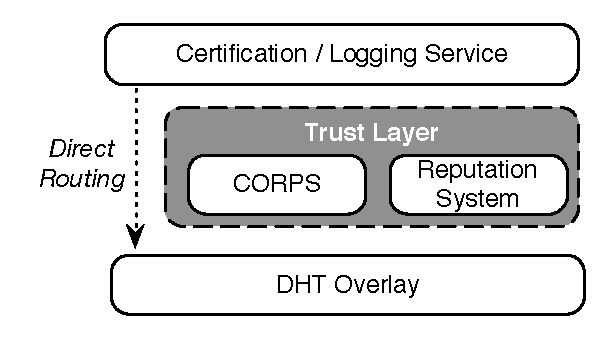
\includegraphics[scale=0.7]{ascent-archi.pdf}
	\end{center}
	\caption{Architecture of our distributed certification service}
	\label{fig:ascent}
\end{figure}

Figure~\ref{fig:log-archi} is a pretty good example of a figure that is completely useless unless it is not accompanied by a textual explanation.

\begin{figure}
	\begin{center}
		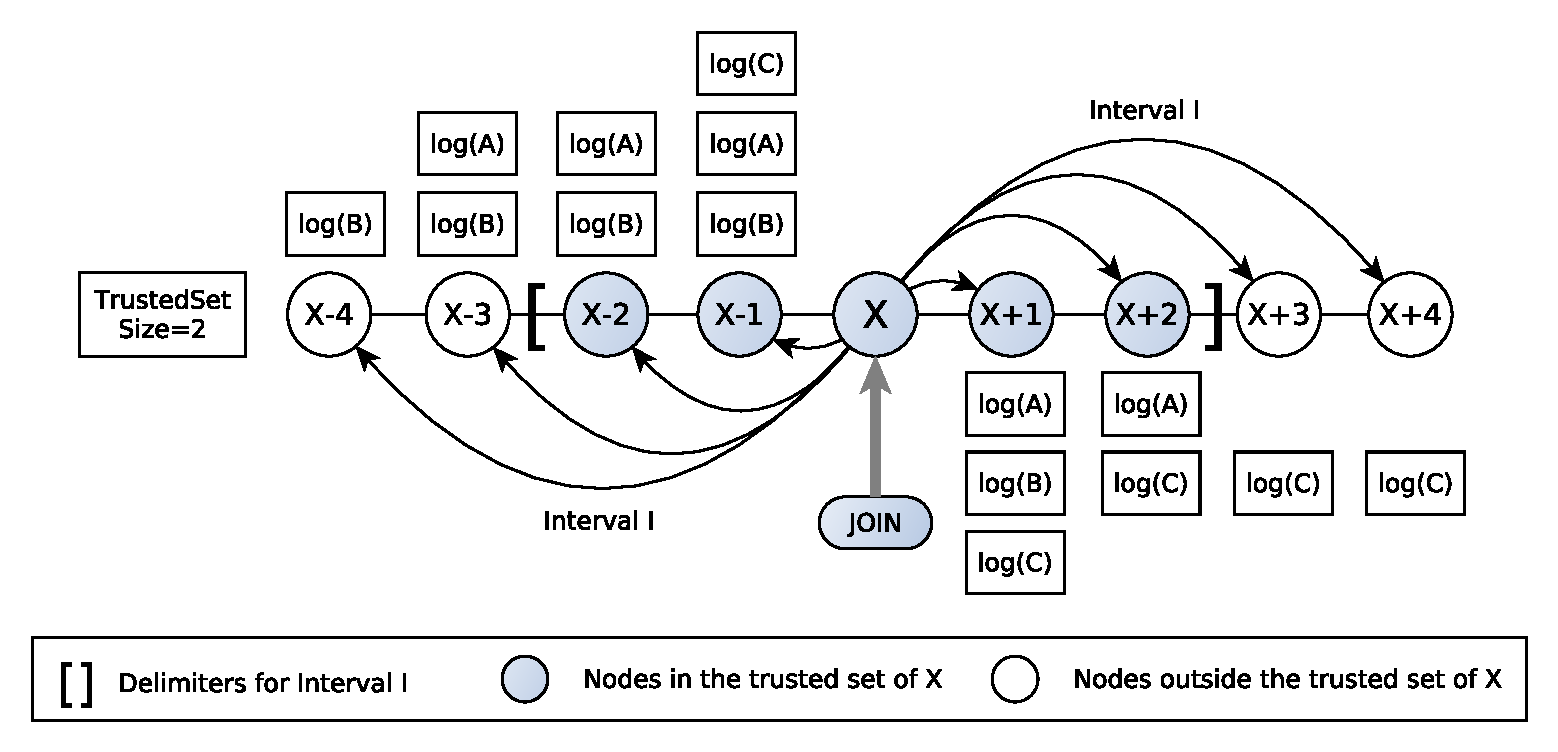
\includegraphics[scale=0.5]{certificates-log-archi.pdf}
	\end{center}
	\caption{Try to guess what this figure illustrates; I double-dare you...}
	\label{fig:log-archi}
\end{figure}

% ------------------------------------------------------------------------------------------------------------------------
\section{Results and Discussion}

The results section details your metrics and experiments for the assessment of your solution. It then provides experimental validation for your approach with visual aids such as data tables and graphs. In particular, it allows you to compare your idea with other approaches you've tested, for example solutions you've mentioned in your related work section.

\subsection{Experimentation protocol}

It is of the utmost importance to describe how you came up with the measurements and results that support your evaluation.

\subsection{Data tables}

Every data table should be numbered, have a brief description as its title, and specify the units used.

As an example, Table~\ref{tab:my_label} compares the average latencies of native application calls to networked services. The experiments were conducted on an Apple MacBook Air 2010 with a CPU speed of 1.4GHz and a bus speed of 800MHz. Each data point is a mean over 20 instances of each call, after discarding both the lowest and the highest measurement.

\begin{table}[ht]
    \centering
    \begin{tabular}{llr}
\hline
\multicolumn{2}{c}{Network Applications} \\
\cline{1-2}
Service    & Protocol & Latency (\si{\ms}) \\
\hline
DNS         & UDP       & \SI{13.65}{\ms}      \\
            & TCP       & \SI{0.01}{\ms}       \\
NTP         & UDP       & \SI{92.50}{\ms}      \\
SMTP        & TCP       & \SI{33.33}{\ms}      \\
HTTP        & TCP       & \SI{8.99}{\ms}       \\
\hline
\end{tabular}
    \caption{Comparison of latencies between services running on \texttt{localhost}.}
    \label{tab:my_label}
\end{table}

\subsection{Graphs}

Graphs are often the most important information in your report; you should design and plot them with great care. A graph contains a lot of information in a short space. Graphs should be numbered and have a title. Their axes should be labelled, with the quantities and units specified. Make sure that individual data points (your measurements) stand out clearly. And of course, always associate your graph with text that explains your results, and outlines the conclusions you draw from these results.

\begin{figure}
	\begin{center}
		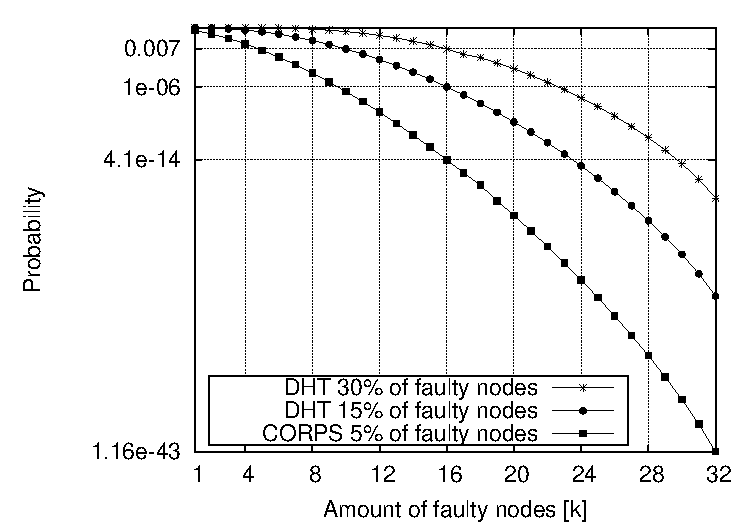
\includegraphics[scale=0.9]{perf-plot-1.pdf}
	\end{center}
	\caption{Probability of including [k] faulty/malicious nodes in the service}
	\label{graph:faulty-proportion-plot}
\end{figure}

For example, Figure~\ref{graph:faulty-proportion-plot} compares the efficiency of three different service architectures in eliminating adversarial behaviors. Every data point gives the probability that $k$ faulty/malicious nodes managed to participate in a computation that involves 32 nodes. In the absence of at least one reliable node ($k = 32$), the failure will go undetected ; but the results show that this case is extremely unlikely, regardless of the architecture. The most significant result pertains to $k = 16$: the reliable nodes detect the failure, but cannot reach a majority to recover. The graph shows that the \texttt{CORPS 5\%} architecture is much more resilient than the \texttt{DHT 30\%} architecture, by a magnitude of $10^{11}$.

% ------------------------------------------------------------------------------------------------------------------------

\section{Discussion}
The discussion section focuses on the main challenges/issues you had to overcome during the project. Outline what your approach does better than the ones you mentioned in your related work, and explain why. Do the same with issues where other solutions  outperform your own. Are there limitations to your approach? If so, what would you recommend towards removing/mitigating them? Given the experience you've gathered working on this project, are there other approaches that you feel are worth exploring?
% ------------------------------------------------------------------------------------------------------------------------

\section{Conclusion}

Give a clear, short, and informative summary of all your important results. Answer the initial question(s) or respond to what you wanted to do, as stated in your introduction. It can be a short table or a list, and possibly one or two short comments or explanations.

Target a reader who may not have time to read the whole report yet, but needs the results or the conclusions immediately. This is a typical situation in real life. Some readers will read your introduction and skip to your conclusion first, and read the whole report only later (if at all).

You may also draw perspectives. What's missing? In what directions could your work be extended?

\bibliographystyle{IEEEtran}
\bibliography{references}


%------ To create Appendix with additional stuff -------%
%\newpage
%\appendix
%\section{Appendix}
%Put data files, CAD drawings, additional sketches, etc.

\end{document} 